\subsection{Software}
A continuación se muestran las pruebas de integración de software realizadas, las cuales se dividieron en tres principales las cuales abarcan una gran mayoría de los casos de uso.
\subsubsection{Prueba de integración 1. Inicio de sesión y consulta de mapa}
Para esta prueba, el flujo definido, empieza con el primer caso de uso que consulta el mapa de gasolineras. Para posteriormente, autenticarse en el sistema y volver a consultar el mapa de gasolineras.\\
En la figura \ref{fig:int1} se puede observar la pantalla de inicio de la aplicación, mostrando las gasolineras cercanas a la ubicación actual (ESCOM).

\begin{figure}[H]
	\centering
	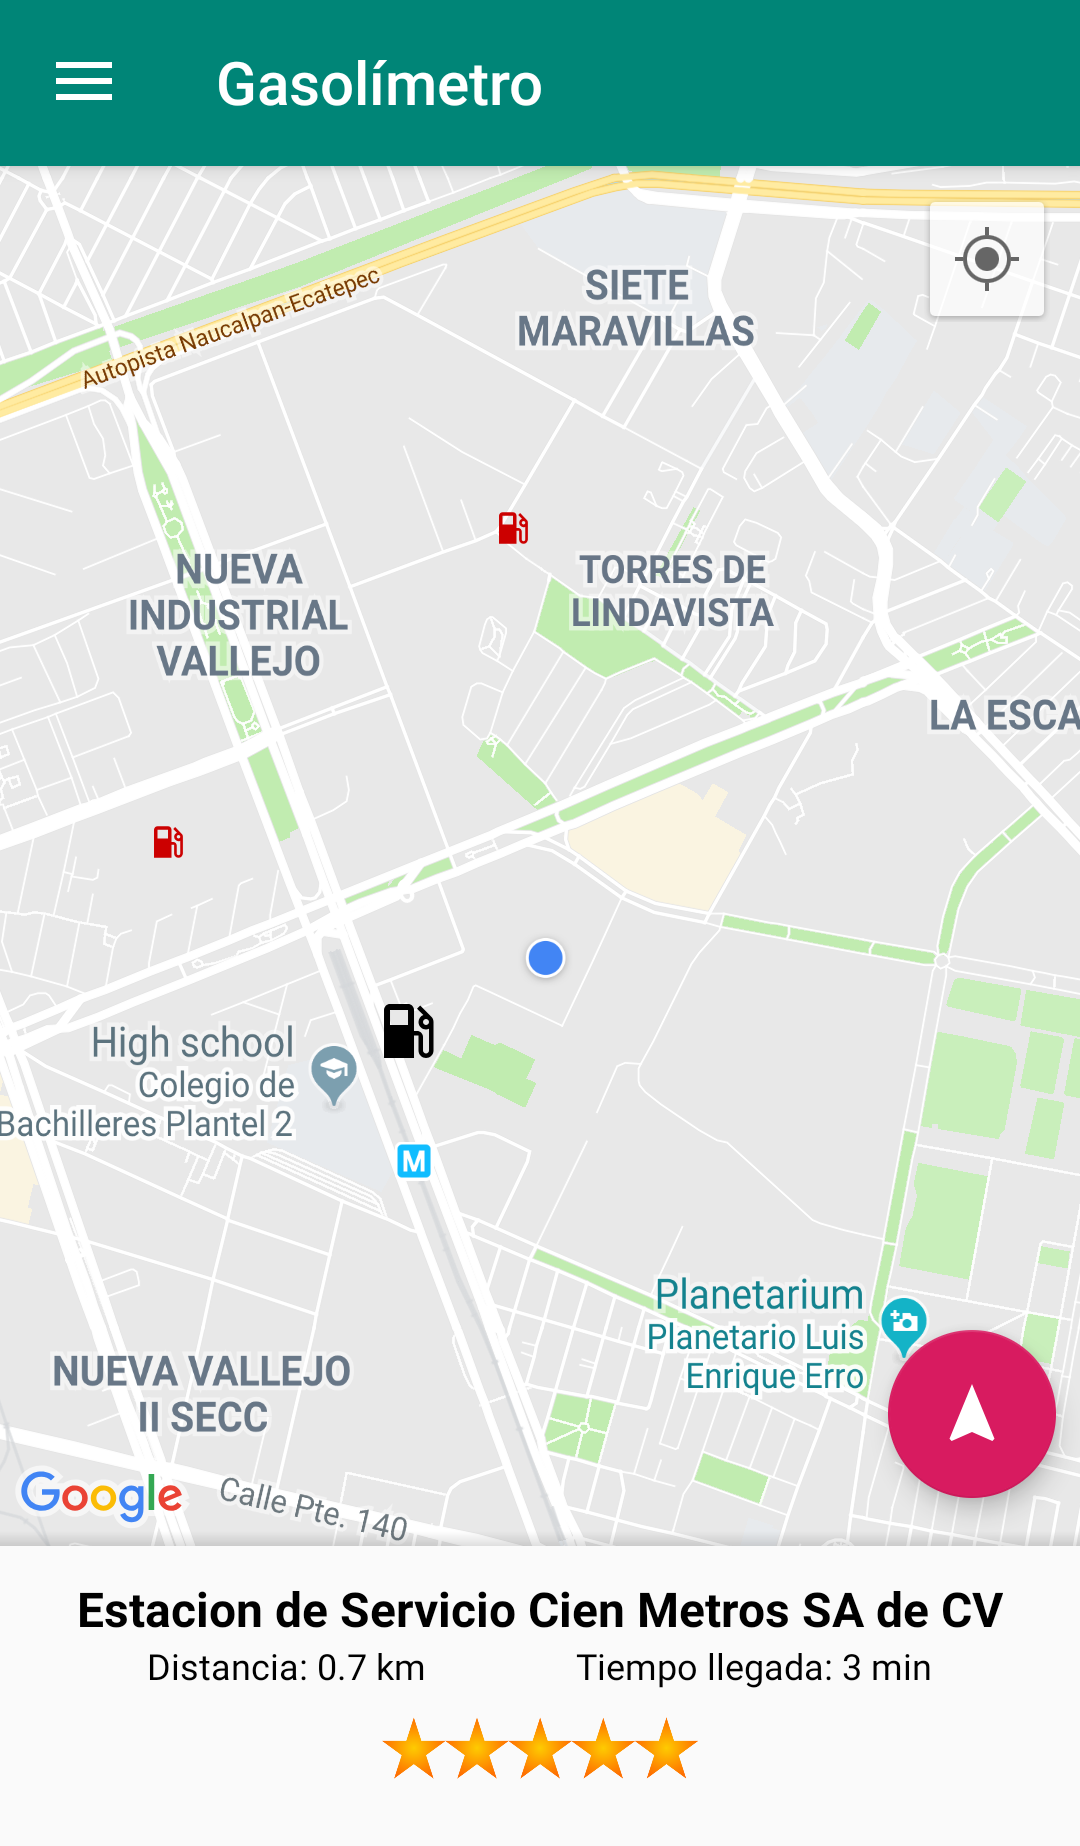
\includegraphics[scale=.2]{DocumentoTecnico/Capitulo6/integracion/Software/images/1.png}
	\caption{Captura de pantalla prueba integración 1 - Consultar mapa (1)}
	\label{fig:int1}
\end{figure}

Posteriormente, se muestra el menú al que tiene acceso un usuario no registrado, con la finalidad de seleccionar la opción ``Iniciar sesión''. Este menú se puede observar en la imagen \ref{fig:int2}

\begin{figure}[H]
	\centering
	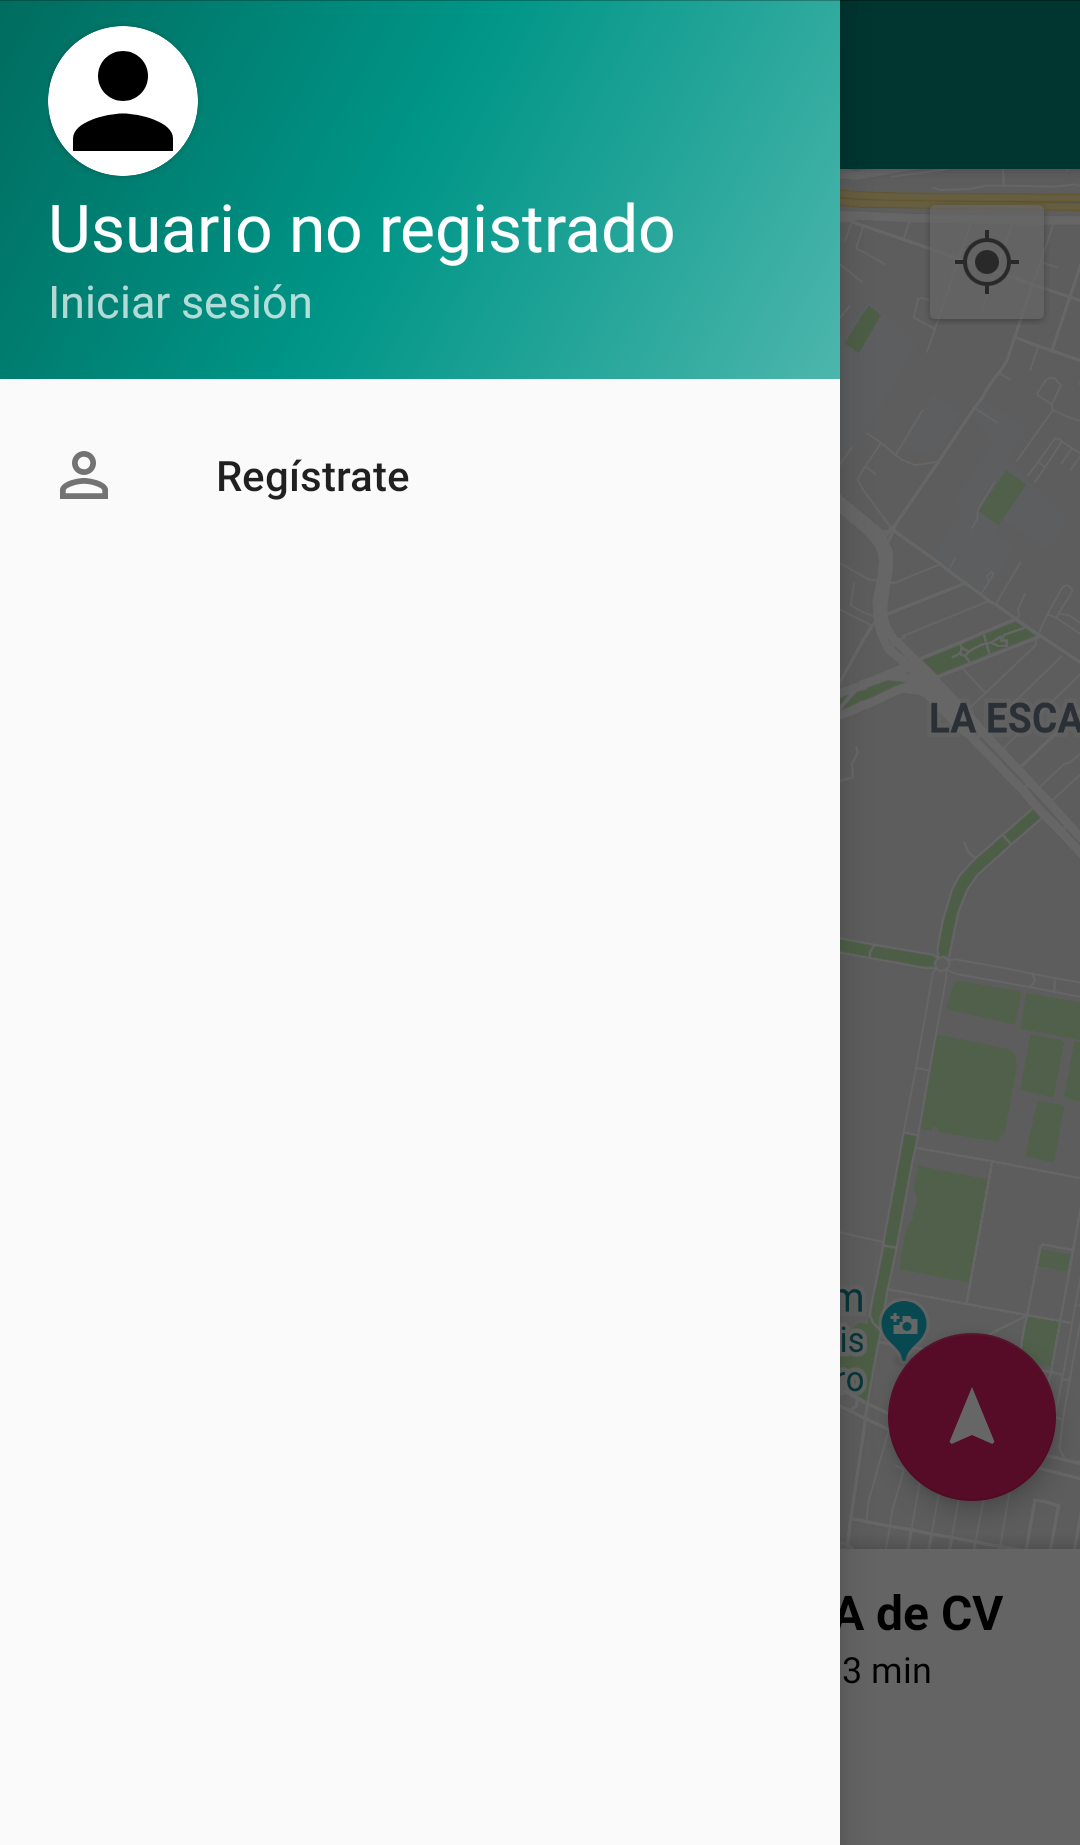
\includegraphics[scale=.2]{DocumentoTecnico/Capitulo6/integracion/Software/images/2.png}
	\caption{Captura de pantalla prueba integración 1 - Menu usuario no registrado}
	\label{fig:int2}
\end{figure}


Cuando la opción ``Iniciar sesión'' es presionada, se muestra una pantalla como la que se muestra en la figura \ref{fig:int3}. En la cual un usuario puede autenticarse.

\begin{figure}[H]
	\centering
	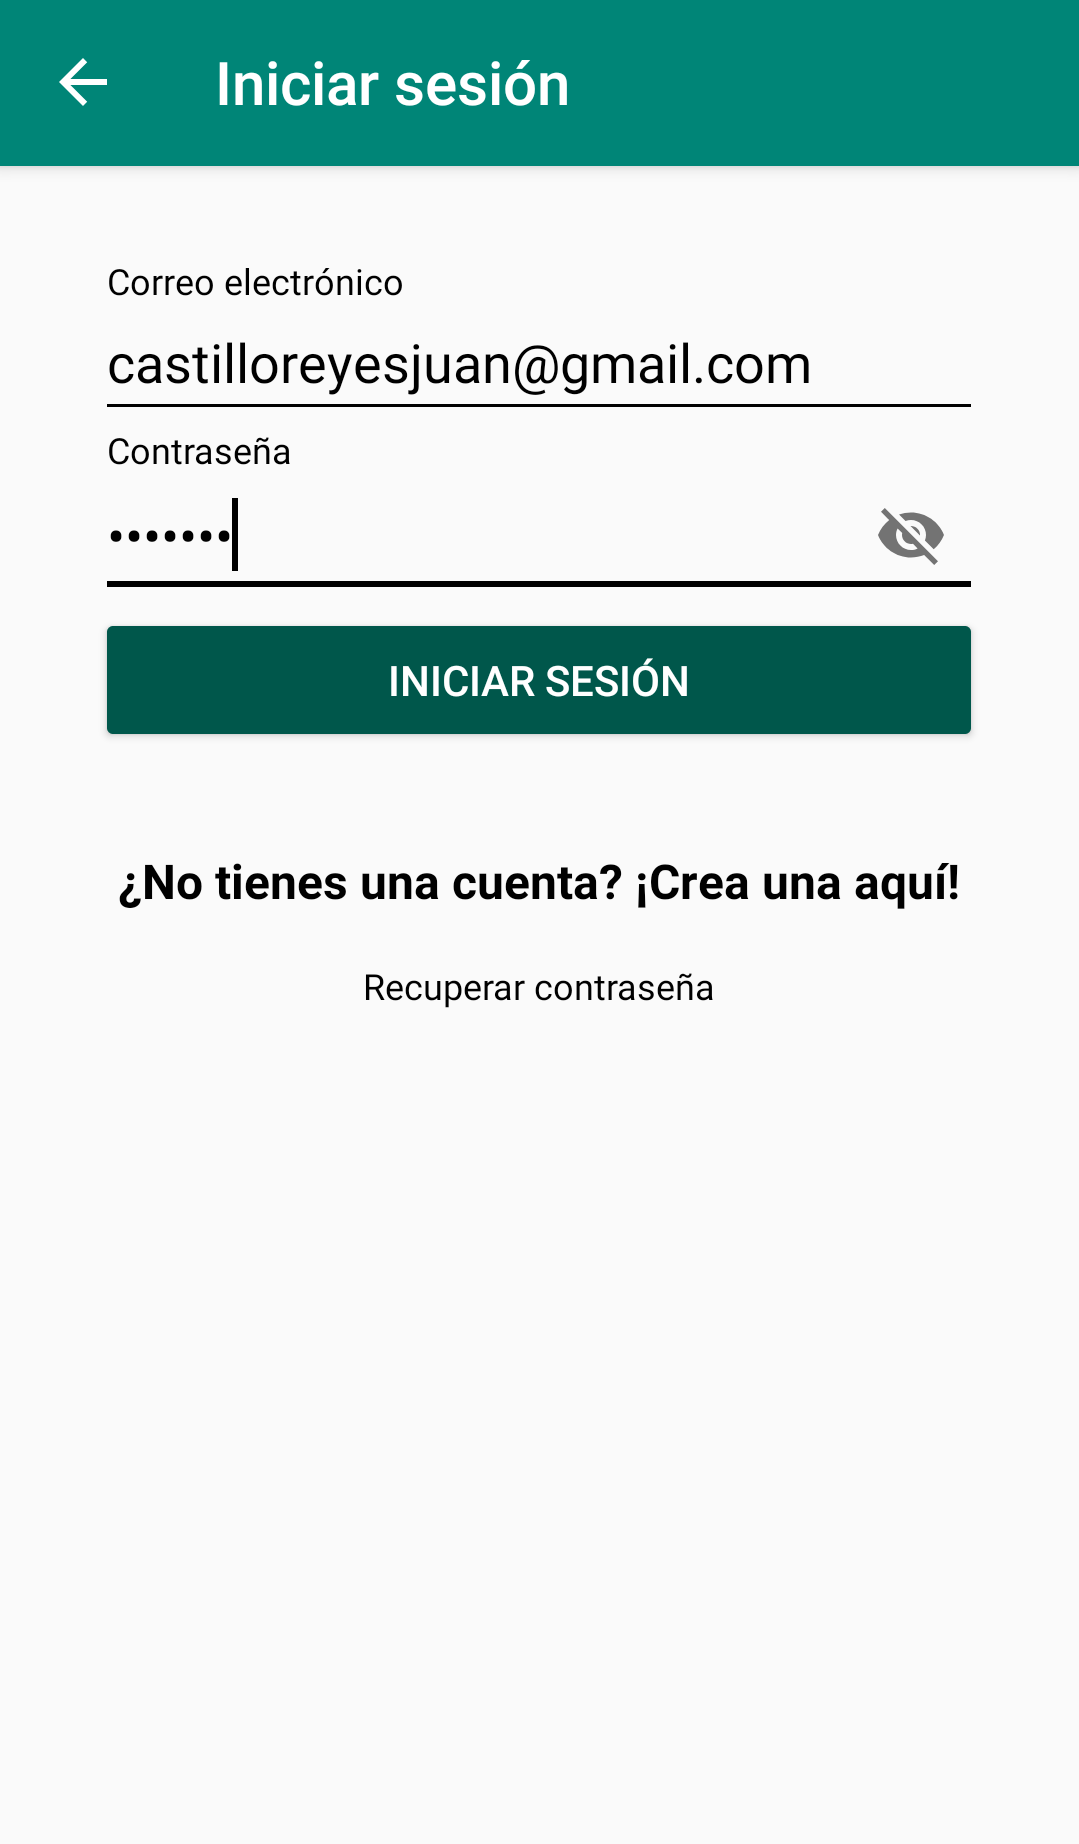
\includegraphics[scale=.2]{DocumentoTecnico/Capitulo6/integracion/Software/images/3.png}
	\caption{Captura de pantalla prueba integración 1 - Autenticar usuario}
	\label{fig:int3}
\end{figure}

Una vez que el usuario llena ambos campos y presiona el botón ``INICIAR SESIÓN'', si su datos son válidos y corresponden al de una cuenta activa, se le mostrará de nueva cuenta el mapa con las gasolineras, como se muestra en la figura \ref{fig:int4}.


\begin{figure}[H]
	\centering
	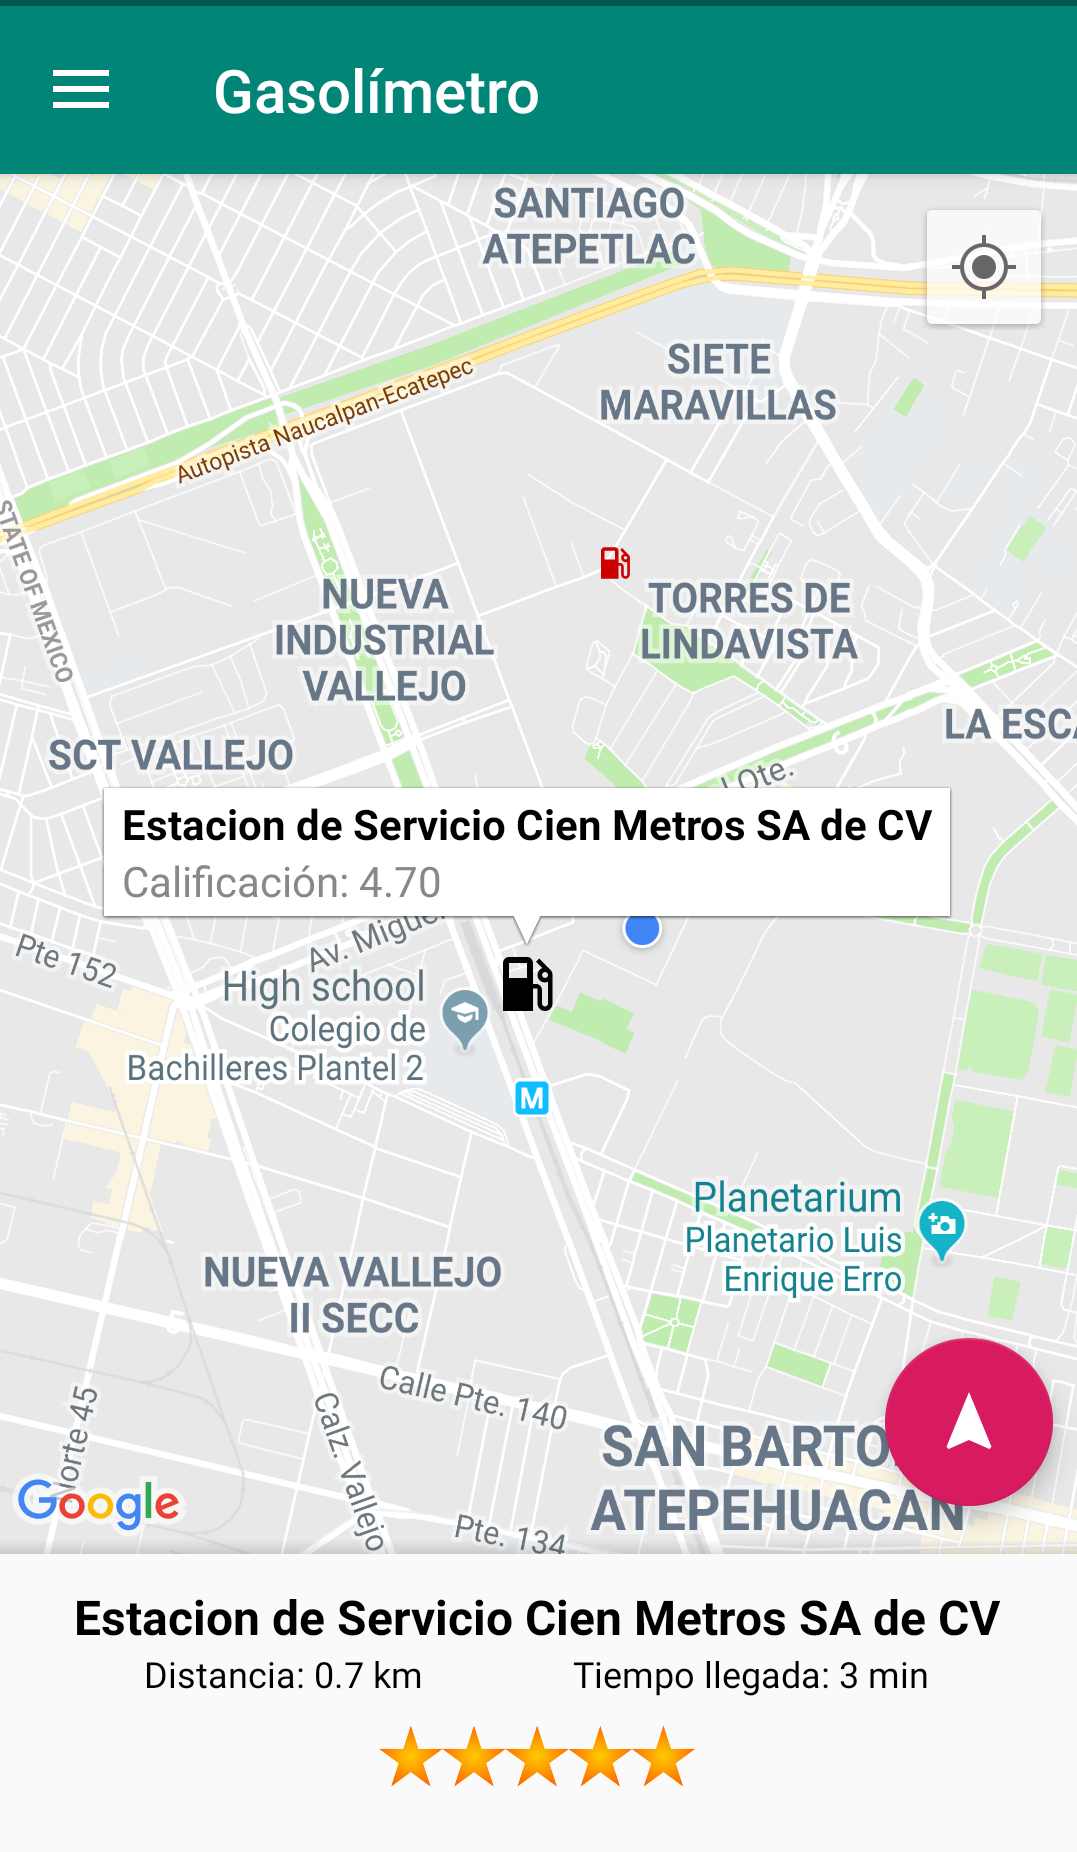
\includegraphics[scale=.2]{DocumentoTecnico/Capitulo6/integracion/Software/images/4.png}
	\caption{Captura de pantalla prueba integración 1 - Consultar mapa (2)}
	\label{fig:int4}
\end{figure}

Con lo cual, podemos concluir que la presente prueba fue exitosa.


\subsubsection{Prueba de integración 2. Envío de medición a servidor}
Para esta prueba, el flujo propuesto fue el siguiente: Dado un usuario con su sesión activa, este debe conectarse al módulo Bluetooth, iniciar una medición de prueba, desconectarse, ingresar la cantidad de litros que le cargaron, y finalmente observar el total de litros que le cargaron de prueba, para que esta medición puede ser almacenada exitosamente.\\

En la figura \ref{fig:int5}, se muestra el menú de un Cliente con cuenta activa, al seleccionar la opción ``Conectar sensor'', empezará el flujo.

\begin{figure}[H]
	\centering
	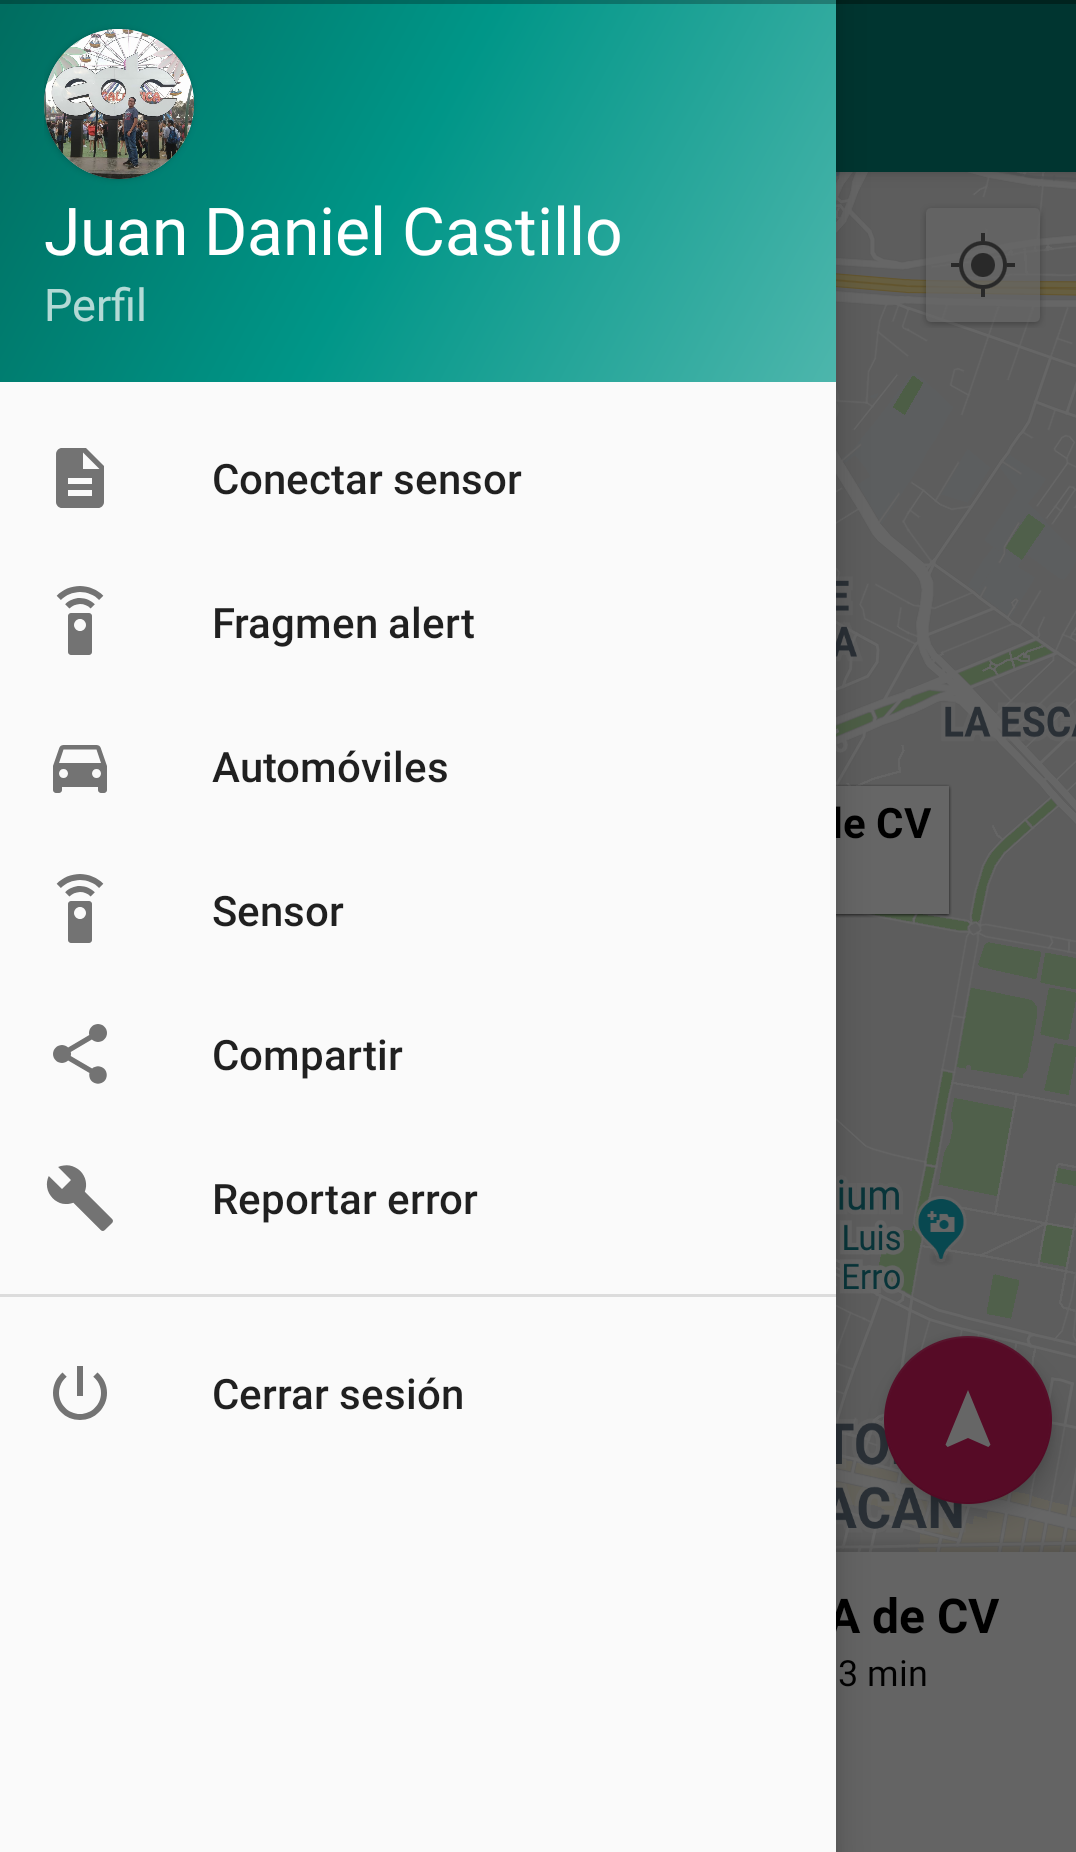
\includegraphics[scale=.2]{DocumentoTecnico/Capitulo6/integracion/Software/images/5.png}
	\caption{Captura de pantalla prueba integración 2 - Menu cliente}
	\label{fig:int5}
\end{figure}

Cuando el usuario presiona la opción ``Conectar sensor'', el sistema verifica que la aplicación móvil pueda conectarse vía Bluetooth al dispositivo, si el teléfono cuenta con esta tecnología pero no está habilitada, se muestra al usuario un mensaje como el que se observa en la figura \ref{fig:int6}, el cual solicita al usuario habilitarlo.

\begin{figure}[H]
	\centering
	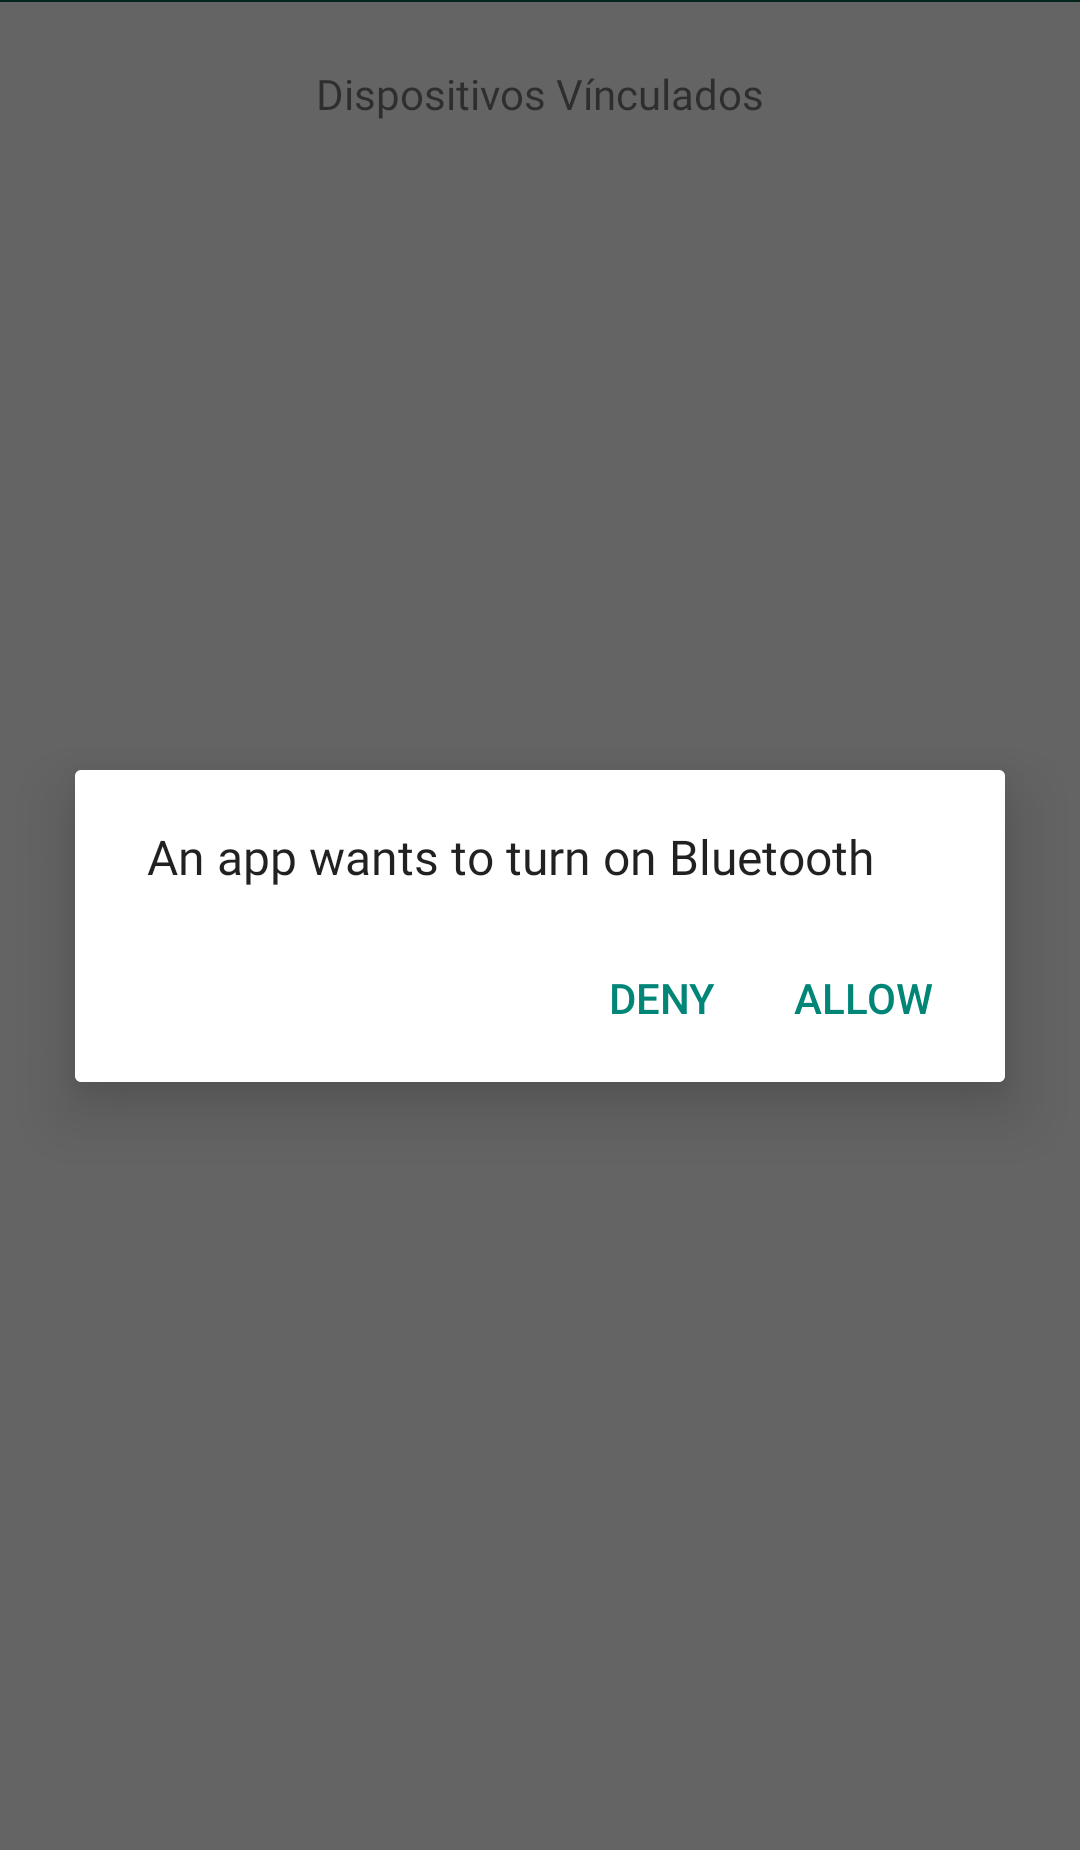
\includegraphics[scale=.2]{DocumentoTecnico/Capitulo6/integracion/Software/images/6.png}
	\caption{Captura de pantalla prueba integración 2 - Solicitud para encender Bluetooth}
	\label{fig:int6}
\end{figure}

Si el usuario habilita el Bluetooth de su teléfono, se muestra una lista con todos los dispositivos Bluetooth a los cuales se ha conectado anteriormente para que seleccione uno, en este caso debe seleccionar el módulo Bluetooth del sensor. Está lista se puede apreciar en la figura \ref{fig:int7}.

\begin{figure}[H]
	\centering
	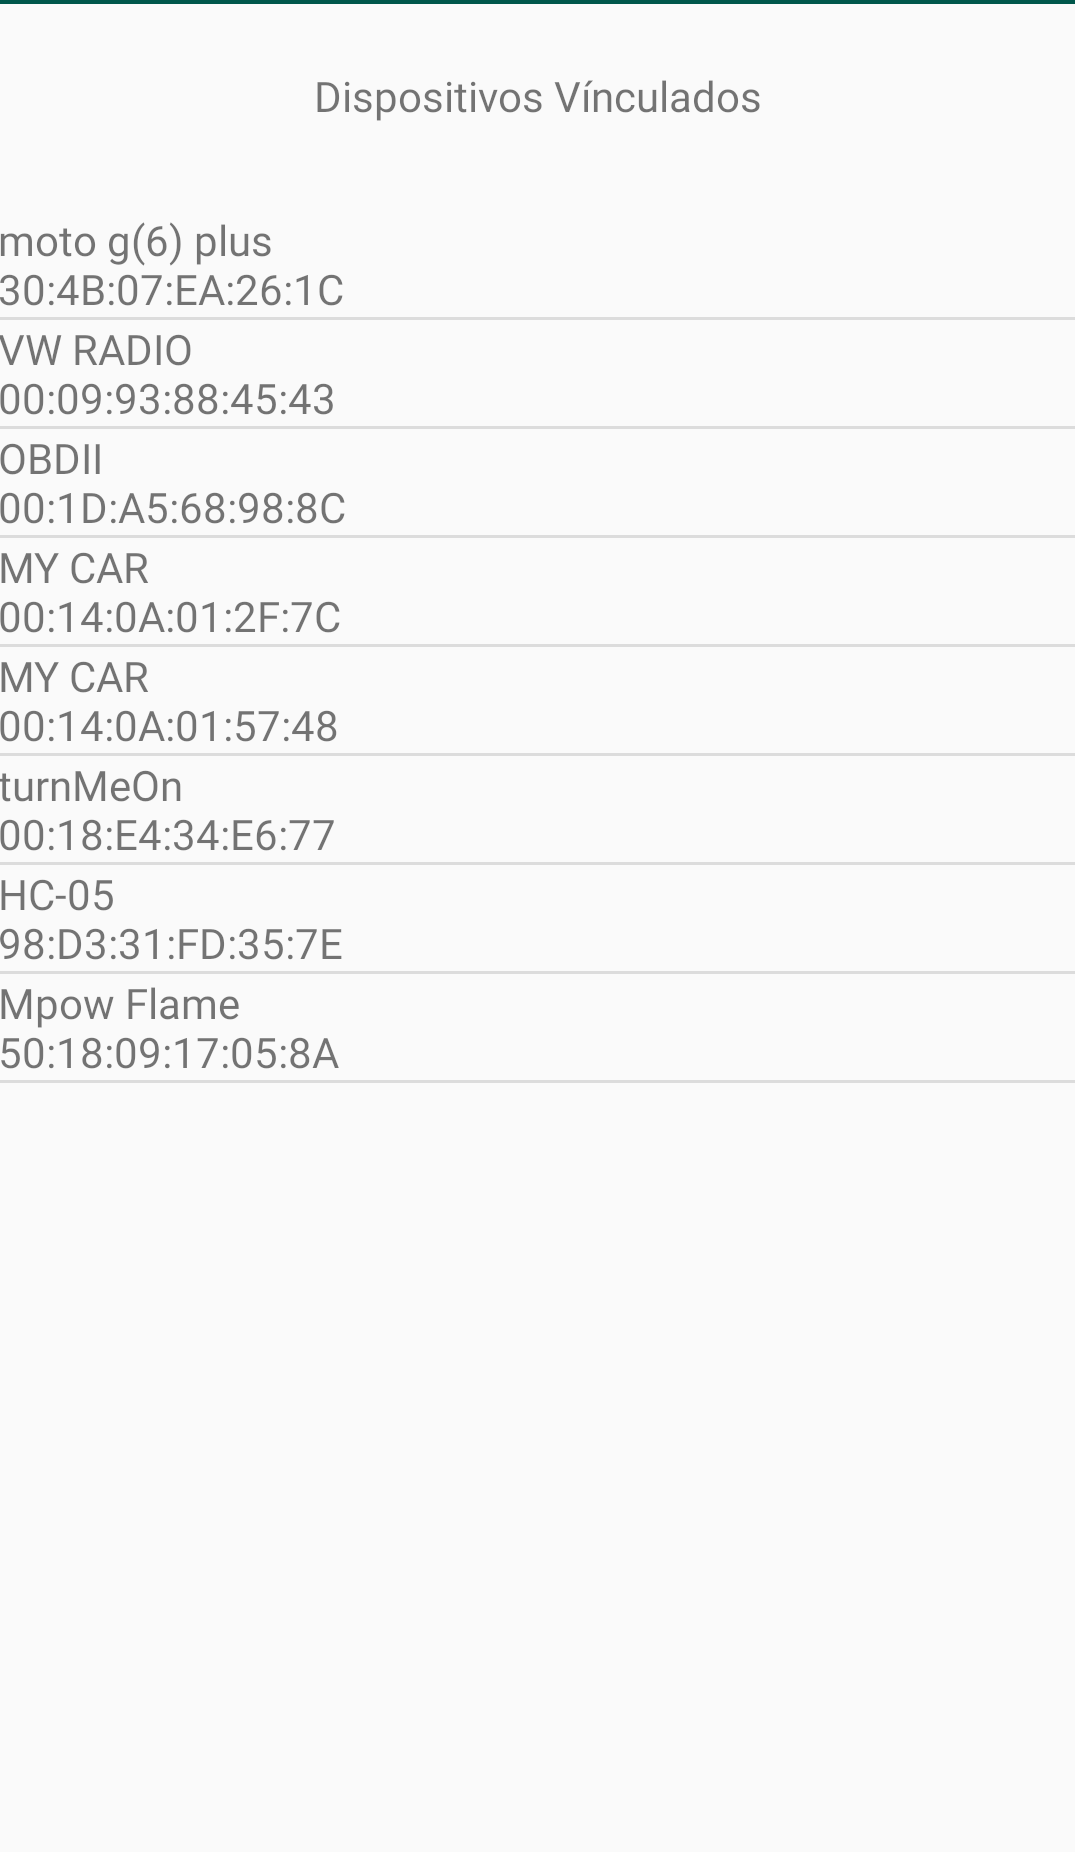
\includegraphics[scale=.2]{DocumentoTecnico/Capitulo6/integracion/Software/images/7.png}
	\caption{Captura de pantalla prueba integración 2 - Seleccionar dispositivo Bluetooth}
	\label{fig:int7}
\end{figure}

Posterior a que el usuario selecciona un elemento de la lista anterior, el usuario vuelve a ver la pantalla principal de la aplicación, dado que la captura de datos enviados por el módulo Bluetooth del sensor se realiza como un servicio que corre de fondo. La pantalla principal se muestra como la de la figura \ref{fig:int8}.

\begin{figure}[H]
	\centering
	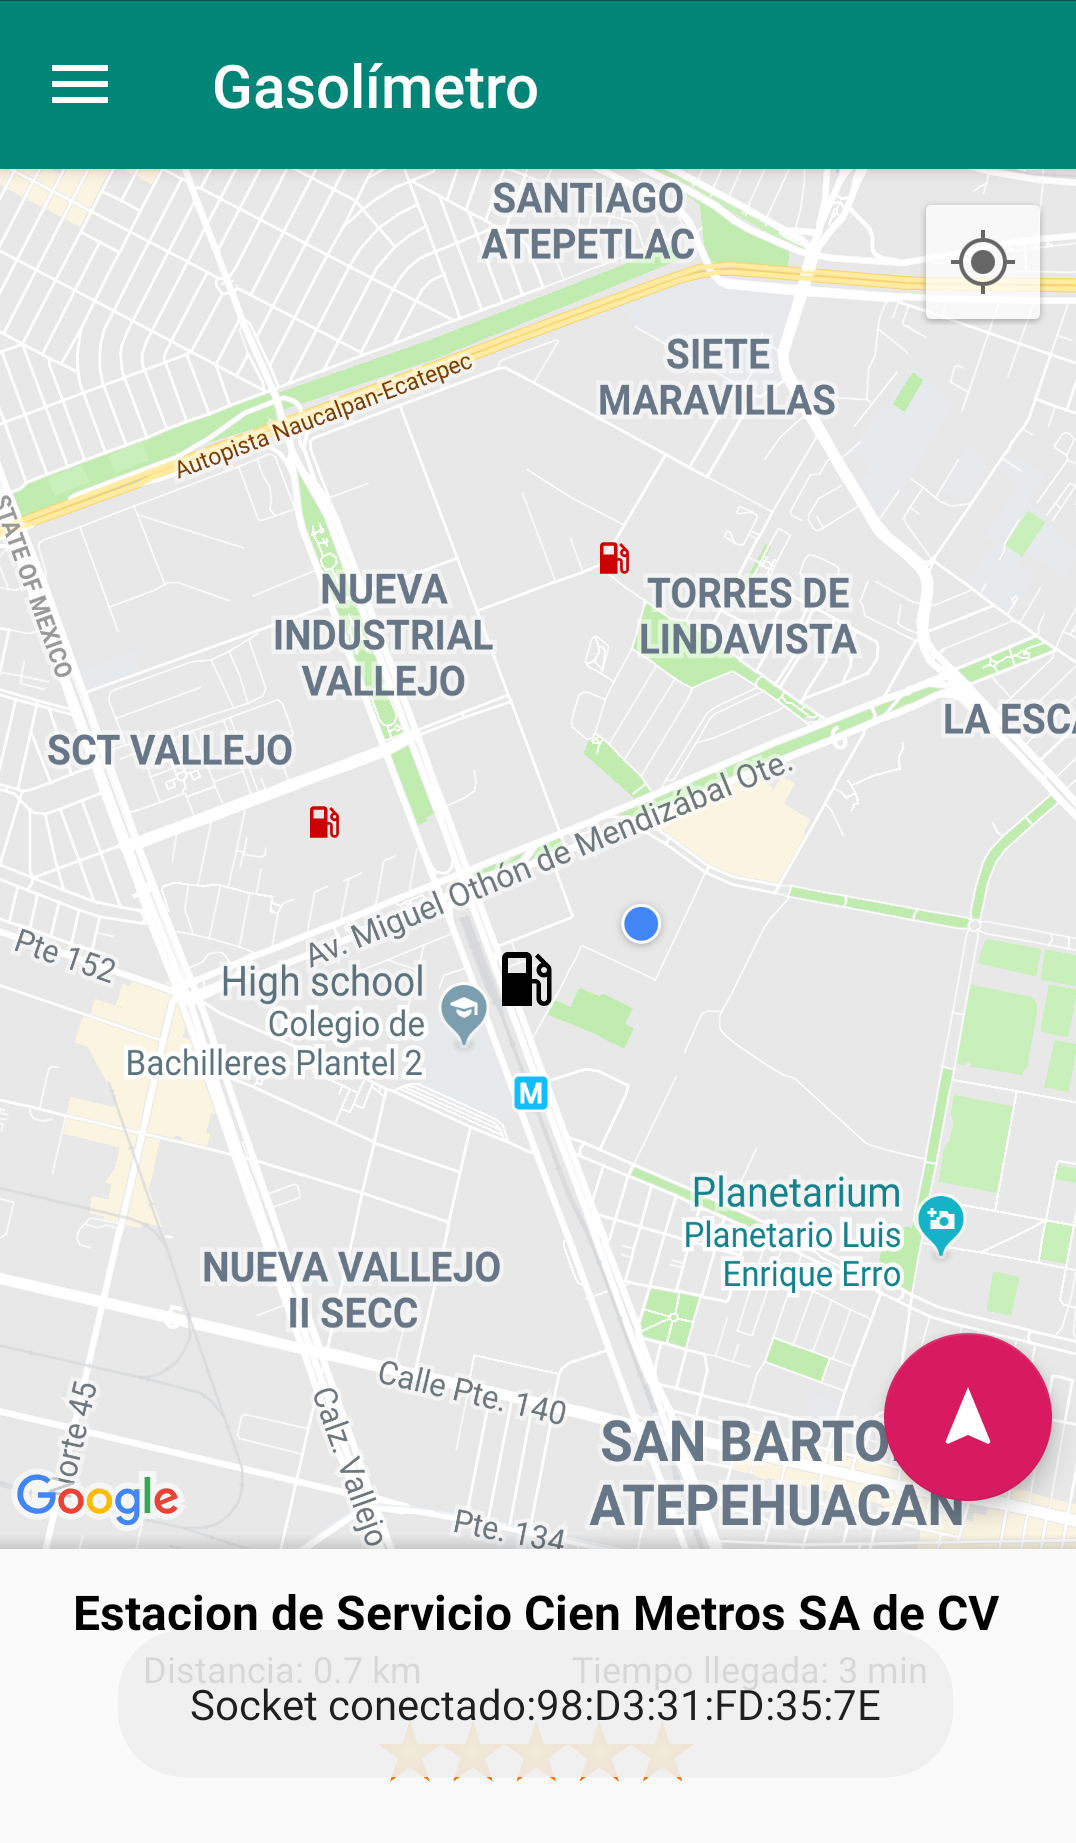
\includegraphics[scale=.2]{DocumentoTecnico/Capitulo6/integracion/Software/images/8.png}
	\caption{Captura de pantalla prueba integración 2 - Mensaje conexión exitosa}
	\label{fig:int8}
\end{figure}

Una vez que se termina de recibir datos, se le muestra una pantalla al usuario solicitando que ingrese la cantidad de litros de gasolina que compro, está pantalla se puede observar en la figura \ref{fig:int9}.

\begin{figure}[H]
	\centering
	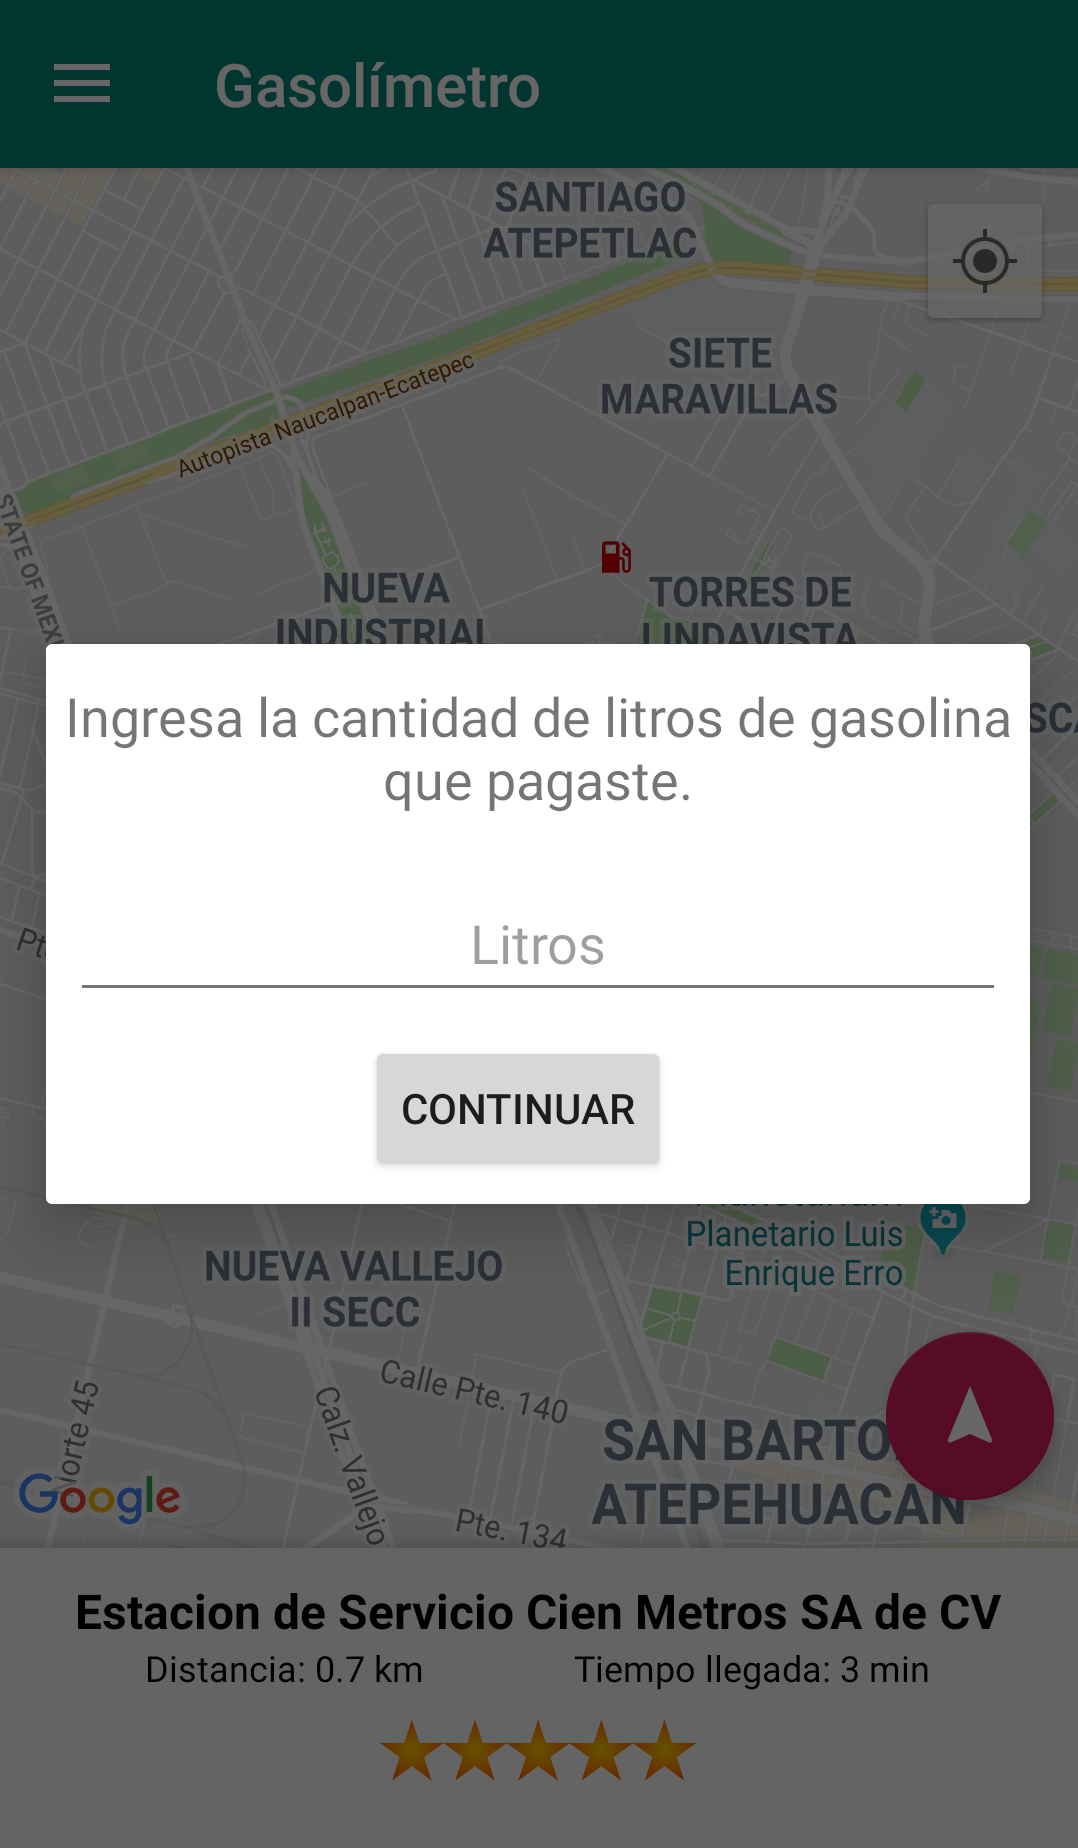
\includegraphics[scale=.2]{DocumentoTecnico/Capitulo6/integracion/Software/images/9.png}
	\caption{Captura de pantalla prueba integración 2 - Solicitar total de gasolina cargada}
	\label{fig:int9}
\end{figure}

Cuando el usuario presiona el botón ``CONTINUAR'' de la pantalla anterior, se muestra la pantalla que se observa en la figura \ref{fig:int10}, la cual le informa de la cantidad de litros que le han sido cargados, al presionar el botón ``ACEPTAR'', la medición es almacenada.

\begin{figure}[H]
	\centering
	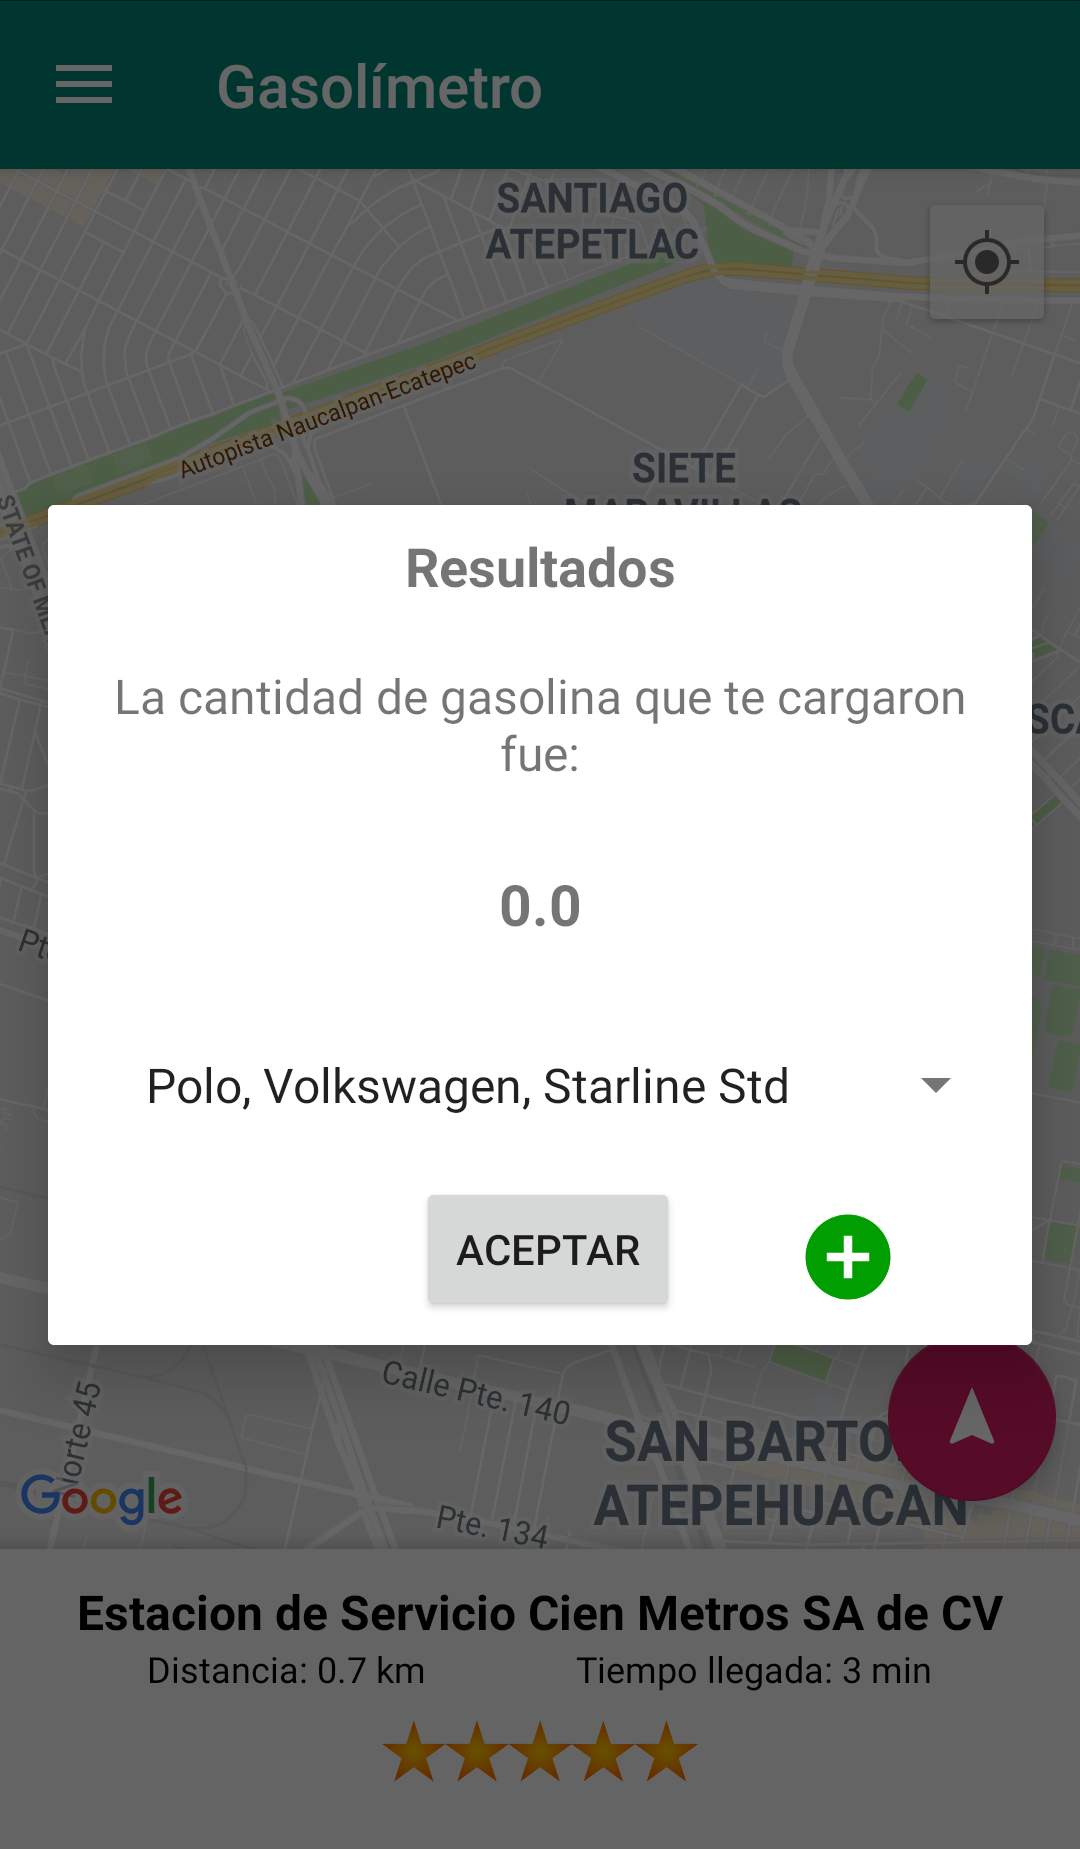
\includegraphics[scale=.2]{DocumentoTecnico/Capitulo6/integracion/Software/images/10.png}
	\caption{Captura de pantalla prueba integración 2 - Mostrar total de gasolina cargada}
	\label{fig:int10}
\end{figure}

Por lo cual, podemos concluir que esta prueba de integración fue exitosa.

\subsubsection{Prueba de integración 3. Consulta de mapa y consulta de ruta de gasolinera}

El flujo propuesto para esta prueba, fue el siguiente: Iniciar la aplicación desde cualquier tipo de usuario, seleccionar una gasolinera distinta a la gasolinera seleccionada en automático, generar un ruta para llegar hasta esta gasolinera.\\

En la figura \ref{fig:int11}, se muestra la pantalla principal de la aplicación, con una gasolinera seleccionada automáticamente, la cual se encuentra de color rojo, debido a que es una gasolinera que no se encuentra en nuestra base de datos, sin embargo, se encuentra en la información que se recibe del API de Google Maps.

\begin{figure}[H]
	\centering
	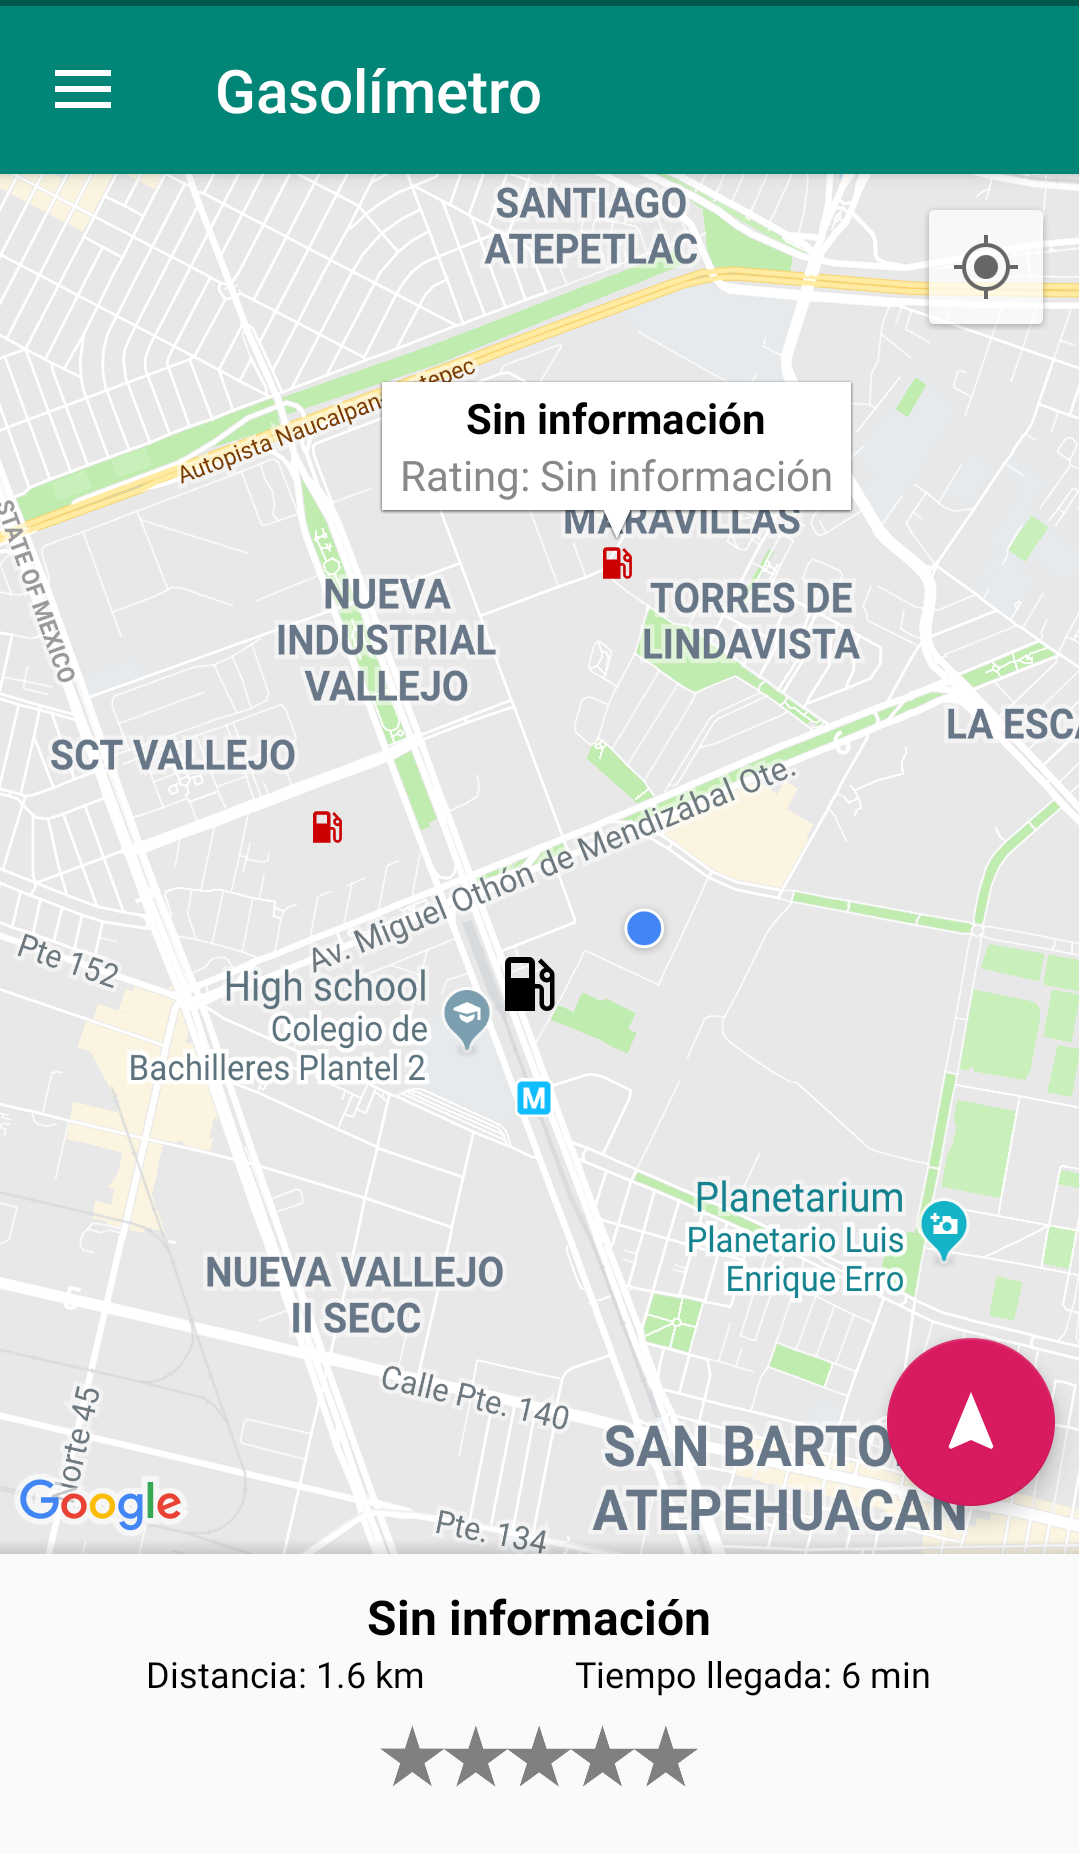
\includegraphics[scale=.2]{DocumentoTecnico/Capitulo6/integracion/Software/images/11.png}
	\caption{Captura de pantalla prueba integración 2 - Selección de gasolinera en consultar mapa}
	\label{fig:int11}
\end{figure}

Posteriormente, se seleccionó la gasolinera ``Estación de Servicio Cien Metros SA de CV'', y se presiona el botón flotante ``¿Cómo llegar?'', el cual genera una ruta de color azul como se puede observar en la figura \ref{fig:int12}.


\begin{figure}[H]
	\centering
	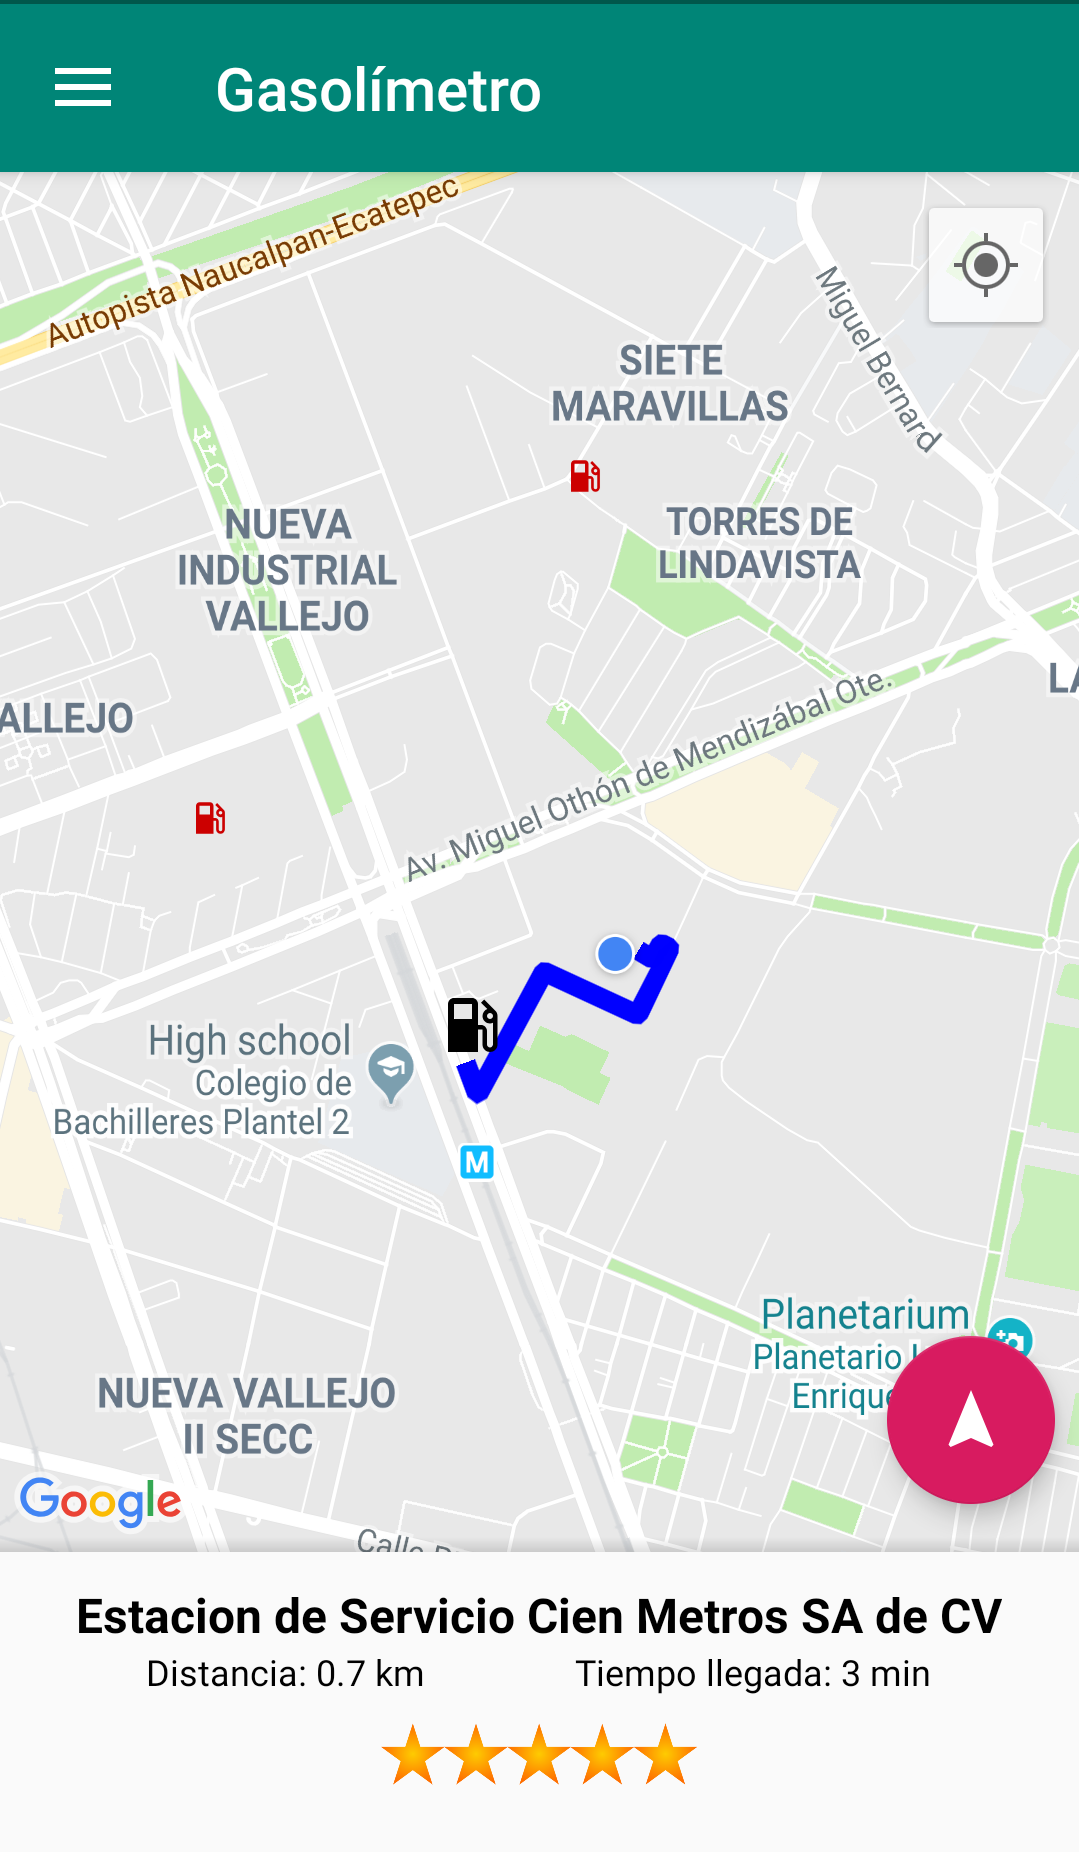
\includegraphics[scale=.2]{DocumentoTecnico/Capitulo6/integracion/Software/images/12.png}
	\caption{Captura de pantalla prueba integración 2 - Realizar recorrido}
	\label{fig:int12}
\end{figure}

Por lo cual, podemos concluir que esta prueba de integración fue exitosa.